\documentclass[11pt,a4paper]{article}
\usepackage[utf8]{inputenc}
\usepackage[T1]{fontenc}

\usepackage[margin=2cm]{geometry}
\usepackage{hyperref}
\usepackage[x11names]{xcolor}
\usepackage{array,multirow,graphicx}
\usepackage{amsmath,amssymb}
\usepackage[boxed]{algorithm2e}
\usepackage{enumitem}
\setlist{itemsep=1pt,topsep=1pt,parsep=1pt,partopsep=1pt}
\usepackage{tikz}
\usetikzlibrary{shapes.geometric}
\usepackage{cleveref}
\usepackage{listings}
\lstdefinestyle{madnklo}{
	basicstyle=\ttfamily\small,
	keywordstyle=\color{Firebrick4},
	commentstyle=\color{RoyalBlue4},
	identifierstyle=\color{black},
	stringstyle=\color{SpringGreen4},
}
\lstset{basicstyle=\ttfamily}

\newcommand{\MadNkLO}[0]{\sc{MadNkLO}}
\newcommand{\py}[1]{\lstinline[language=python]{#1}}

\title{Generation of counterterms in \MadNkLO}
\author{Simone Lionetti}
\date{\today}


\begin{document}

\maketitle

This document describes the contents of the file \texttt{subtraction.py}
(located in \texttt{madgraph/core}).


\section{Classes}


\subsection{\py{SubtractionLeg}}
\label{ssec:subtractionleg}

For the purpose of the subtraction,
it is impractical to carry around the whole information
that is contained in an object of the type \py{base_objects.Leg}.
A simpler object \py{SubtractionLeg} is therefore defined
with the following three attributes:
\begin{itemize}
	\item \py{n}: an integer that indicates the leg number in the process,
	\item \py{pdg}: the PDG identifier which specifies the type of particle,
	\item \py{state}: a flag to specify if the leg
		is in the initial or in the final state.
\end{itemize}

For convenience, a class \py{SubtractionLegSet} which represents
a set of \py{SubtractionLeg}'s is also implemented.
Internally, this is just a sorted \py{tuple} since it is assumed
that order is irrelevant.
However, this object also provides some additional useful methods.


\subsection{\py{SingularStructure}}
\label{ssec:singularstructure}

The \py{SingularStructure} class is designed to identify
unresolved limits in phase space, and by extension counterterms.
It is a recursive structure which represents a tree of \py{SubtractionLeg}'s
in a process.
At each level, the leaves are gathered
into a \py{SubtractionLegSet} attribute called `\py{legs}'
and the \py{SingularStructure} that specify sub-trees are grouped
into a \py{list} called `\py{substructures}'.
There are currently three classes that inherit from \py{SingularStructure}
and represent different unresolved limits:
\begin{itemize}
	\item \py{SoftStructure} indicates that all of its sub-legs are soft,
	\item \py{CollStructure} indicates
		that all of its sub-legs are collinear,
	\item \py{BeamStructure} specifies that a leg is taken from a hadron
		beam after some splitting.
\end{itemize}
The generic parent class \py{SingularStructure} can be instantiated
to group together several structures and specify an additional set of legs;
this feature is exploited in the implementation of momentum mappings
to identify which particles to recoil against.

\begin{figure}
\centering
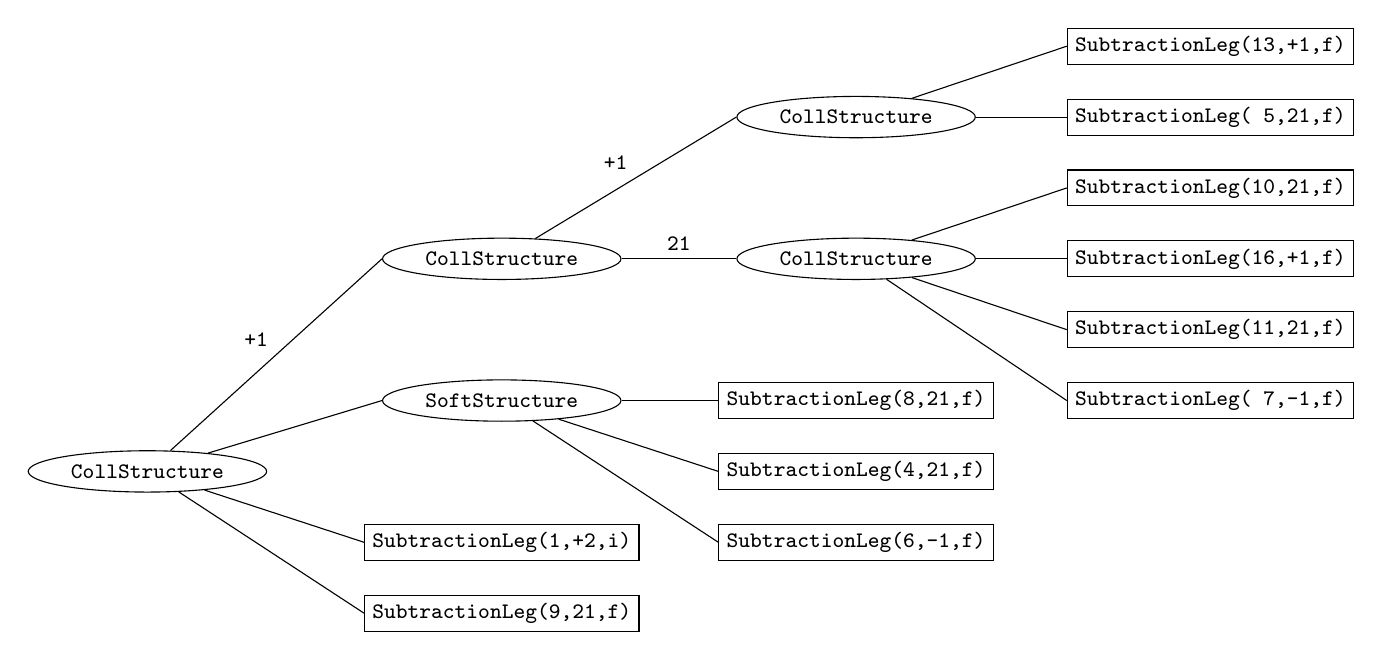
\begin{tikzpicture}[scale=0.9]
\footnotesize
	\draw (0,  0) node[ellipse,draw] (C1)  {\tt{CollStructure}};
	\draw (5, +3) node[ellipse,draw] (C2)  {\tt{CollStructure}};
	\draw (5, +1) node[ellipse,draw] (S2)  {\tt{SoftStructure}};
	\draw (10,+3) node[ellipse,draw] (C3a) {\tt{CollStructure}};
	\draw (10,+5) node[ellipse,draw] (C3b) {\tt{CollStructure}};
	\draw (5, -1) node[draw] (leg2a) {\tt{SubtractionLeg(1,+2,i)}};
	\draw (5, -2) node[draw] (leg2b) {\tt{SubtractionLeg(9,21,f)}};
	\draw (10,-1) node[draw] (leg3a) {\tt{SubtractionLeg(6,-1,f)}};
	\draw (10, 0) node[draw] (leg3b) {\tt{SubtractionLeg(4,21,f)}};
	\draw (10,+1) node[draw] (leg3c) {\tt{SubtractionLeg(8,21,f)}};
	\draw (15,+1) node[draw] (leg4a) {\tt{SubtractionLeg( 7,-1,f)}};
	\draw (15,+2) node[draw] (leg4b) {\tt{SubtractionLeg(11,21,f)}};
	\draw (15,+3) node[draw] (leg4c) {\tt{SubtractionLeg(16,+1,f)}};
	\draw (15,+4) node[draw] (leg4d) {\tt{SubtractionLeg(10,21,f)}};
	\draw (15,+5) node[draw] (leg4e) {\tt{SubtractionLeg( 5,21,f)}};
	\draw (15,+6) node[draw] (leg4f) {\tt{SubtractionLeg(13,+1,f)}};
	\draw (C1) edge node[above left] {\tt{+1}} (C2.west);
	\draw (C1) edge (S2.west);
	\draw (C1) edge (leg2a.west);
	\draw (C1) edge (leg2b.west);
	\draw (S2) edge (leg3a.west);
	\draw (S2) edge (leg3b.west);
	\draw (S2) edge (leg3c.west);
	\draw (C2) edge node[above] {\tt{21}} (C3a.west);
	\draw (C2) edge node[above left] {\tt{+1}} (C3b.west);
	\draw (C3a) edge (leg4a.west);
	\draw (C3a) edge (leg4b.west);
	\draw (C3a) edge (leg4c.west);
	\draw (C3a) edge (leg4d.west);
	\draw (C3b) edge (leg4e.west);
	\draw (C3b) edge (leg4f.west);
\end{tikzpicture}
\caption{
Example scheme of a \py{SingularStructure} object.
The nodes in bubbles belong to the list of \py{substructure}
of the structure they are linked to on the left,
while the ones in boxes belong to its \py{legs}.
Within \py{SubtractionLeg} objects, initial and final states
are here abbreviated with the letters \py{i} and \py{f} respectively.
}
\label{fig:singularstructure}
\end{figure}

For the sake of concreteness,
a non-trivial example of \py{SingularStructure}
is illustrated in \cref{fig:singularstructure}.
In the conversion to a string,
\py{SingularStructure}'s are converted to a single character,
and the PDG codes and the state labels
of \py{SubtractionLeg}'s are suppressed,%
\footnote{
This is the default behaviour,
the printout can be tuned by calling the function
\py{__str__()} explicitly
and passing the keyword arguments
\py{print_n}, \py{print_pdg} and \py{print_state}.
}
such that the object of \cref{fig:singularstructure} prints as
\begin{equation}
	\texttt{C(C(C(5,13),C(7,10,11,16)),S(4,6,8),1,9)}.
\end{equation}
The conversion of objects to characters is carried out
through the method \py{name()}, according to the rules
\begin{equation}
\label{eq:singularnames}
\begin{aligned}
	&\text{\py{SingularStructure}} \to \texttt{`'}, &
	&\text{\py{CollStructure}} \to \texttt{`C'}, \\
	&\text{\py{SoftStructure}} \to \texttt{`S'}, &
	&\text{\py{BeamStructure}} \to \texttt{`F'}.
\end{aligned}
\end{equation}
Whenever the species of particles and their state are not relevant
or clear from the context, we will identify \py{SingularStructure}'s
using their printout for brevity.

In order to understand how limits are specified using these objects,
let us consider some simpler examples.
While the \py{SingularStructure} \texttt{C(3,5,7,8)}
indicates the limit where legs number 3, 5, 7 and 8
are simultaneously taken to be collinear,
\texttt{(C(3,5),C(7,8))} denotes the limit
where 3 goes collinear to 5, and 7 to 8.%
\footnote{
Note that the outermost bracket around the latter printout
denotes a \py{SingularStructure} of unspecified type,
as indicated in \cref{eq:singularnames}.
Although the default behaviour does not distinguish among
different orderings of the limits which appear at the same level,
this can be tweaked using the keyword argument \py{orderless}
of the comparison function \py{__eq__} for \py{SingularStructure}.
}
These situations are still distinct from the nested limit
\texttt{C(C(3,5),7,8)}, which approaches the configuration
where all four particles are collinear
by first letting legs 3 and 5 go to the same direction,
and subsequently sending the angles among their common parent,
leg 7 and 8 to zero.
Similarly, \texttt{S(C(4,7))} indicates the limit
of legs 4 and 7 going collinear to each other,
and their parent leg subsequently going soft.


\subsection{\py{Current}}


\subsection{\py{Counterterm}}


\subsection{\py{IRSubtraction}}


\section{Generation of local counterterms}
\label{sec:generation}

\subsection{Listing elementary structures}
\label{ssec:elementary}

Given a process, the first step towards constructing
a local infrared subtraction is to enumerate
all of the different unresolved limits which potentially need to be regulated.
In order to achieve this, we start with the identification of all possible
\emph{elementary} limits of a single set of particles
simultaneously approaching a singular configuration.
In practice, this corresponds to a set of particles
which are either all soft or all collinear to each other,
and may be represented by a \py{SingularStructure} of the appropriate type
with no substructure.

After an \py{IRSubtraction} module has been initialised
with the appropriate model and couplings specifications,
a list of all relevant elementary structures can be obtained
by calling the method \py{get_all_elementary_structures()}
on a \py{base_objects.Process} instance \py{process}
for a given maximum number \py{max_unresolved} of unresolved particles.
Internally, the generation proceeds as follows:
\begin{algorithm}[H]
\For{$n=1$ to \emph{\py{max_unresolved}}}{
	\For{each combination of $n$ final-state legs}{
		\If{the combination can become soft}{
			add its soft structure to the list\;
		}
	}
	\For{each combination of $n+1$ final-state legs}{
		\If{the combination can become collinear}{
		add its collinear structure to the list\;
		}
	}
	\For{each combination of $n$ final-state legs}{
		\For{each hadronic initial-state leg}{
			\If{the set of these $n+1$ legs can become collinear}{
				add its collinear structure to the list\;
			}
		}
	}
}
\end{algorithm}
The conditional statements about whether a set of particles
can become soft or collinear are implemented in the methods
\py{can_become_soft()} and \py{can_become_collinear()} of \py{IRSubtraction}.
They determine the candidate parent particles of the given legs
using \py{parent_PDGs_from_legs()}.%
\footnote{
Note that in principle there might be more than one possible parent,
as for instance in the case of a $q\bar{q}$ pair
which might be produced from a gluon or a photon.
}


\subsection{Nesting structures}
\label{ssec:nest}

Lists of elementary structures can be assembled into nested structures
of the type described in \cref{ssec:singularstructure},
which are arguably more practical to process counterterms.
This is achieved by grouping the list
under a \py{SingularStructure} of unspecified type,
and calling the method \py{nest()} on it.
In turn, this relies on \py{act_on()}.

Moreover, all possible combinations can be formed
from a list of elementary structure using the method \py{get_all_combinations}
of \py{SingularStructure}.


\subsection{Assembling counterterms}
\label{ssec:counterterms}

\begin{thebibliography}{9}

\end{thebibliography}

\end{document}
